\section{Vorstellung: Algorithmen}

Approximative Algorithmen dienen jeweils sehr spezifischen Aufgaben, die in einem großen Datensatz oder Stream gelöst werden können.
Da Probleme wie das Zählen unterschiedlicher Elemente oder das bestimmen eines häufigsten Elements mathematisch sehr unterschiedliche Herangehensweisen erfordern, können diese Algorithmen also nur für ein spezielles Aufgabengebiet eingesetzt werden.
Hier sollen einige Algorithmen mit unterschiedlichen Einsatzgebieten und deren Funktionsweisen grob vorgestellt werden, um einen Überblick über verschiedene Aufgabenbereiche und deren Lösungen zu bieten.

\subsection{HyperLogLog}

Der HyperLogLog-Algorithmus basiert auf dem Flajolet-Martin-Algorithmus, welcher erst von Durand und Flajolet \cite{durand2003} zum LogLog-Algorithmus und schließlich von Flajolet et al. \cite{flajolet2007} zum HyperLogLog-Algorithmus weiterentwickelt wurde.
Der Algorithmus dient der approximativen Lösung des sog. Count-Distinct-Problems, bei dem es die Anzahl unterschiedlicher, auftretender Elemente zu zählen gilt.
Da die naive Lösung dieses Problems, die Speicherung in einer Menge und das Auslesen deren Länge, bei großen Datenmengen zu einem stetig steigenden Speicherplatzbedarf führt, ist eine speicherplatzeffiziente Lösung mit annähernd korrektem Ergebnis vorzuziehen.

Dieses Problem wurde schon in der ersten Version des Algorithmus gelöst und seitdem stetig weiterentwickelt.
So konnte der Speicherbedarf bei der Weiterentwicklung des LogLog- zum HyperLogLog-Algorithmus um 64\% gesenkt werden, ohne dabei Präzision des Ergebnisses einzubüßen \cite{flajolet2007}.

Die Funktionsweise des HyperLogLog-Algorithmus wird in \autoref{sec:proof-of-concept-funktionsweise} detaillierter behandelt und deswegen hier nicht weiter beschrieben.

\subsection{T-Digest}

Der T-Digest ist ein von Ted Dunning entwickelter Algorithmus zum approximieren der Verteilung von Daten mit Quantilen \cite{dunning2019}.

Quantile sind Schwellenwerte auf einer Verteilungsfunktion, die für einen gegebenen Prozentsatz angeben, welche Werte unterhalb dieses Schwellenwerts liegen.
So liefert das 25\%-Quantil beispielsweise den Wert, für den gilt, dass 25\% aller Werte in der zugrundeliegenden Datenmenge kleiner sind als dieser Wert.
Das 50\%-Quantil entspricht somit dem Median einer Datenmenge -- dem Wert, der genau in der Mitte der geordneten Liste steht.

Bei einer naiven Lösung dieser Aufgabe müssen alle eingehenden Daten in einer Liste gespeichert und geordnet werden, woraufhin anschließend die Quantilen ausgelesen werden können.
Beim T-Digest wird die Verteilung der Daten auf wichtige Punkte, in deren Umgebung viel Veränderung stattfindet, heruntergebrochen \cite{davidsonpilon2015}.
Diesen Schwerpunkten (engl. Centroids) wird ein Gewicht zugewiesen, woraus sich später eine gute Approximation der Verteilung ableiten lässt.
Laut Dunning \cite{dunning2015} ist hierbei eine höhere Präzision vor allem in den Randbereichen der Verteilung von besonderer Wichtigkeit.
So sei eine Abweichung von etwa 0,5\% im Bereich des Medians in Ordnung, in Extremfällen wie dem 99,99\%-Quantil jedoch nicht mehr, da es hier darauf ankommt, einen sehr kleinen Bereich zu identifizieren.
Die Verteilung der Gewichte auf Schwerpunkte und das Auslassen von Punkten ist in \autoref{fig:t-digest} dargestellt.
In diesem Beispiel wurden 100\,000 zufällige Zahlen im Bereich von 1 bis 1\,000, deren Verteilung links zu sehen ist, durch den T-Digest Algorithmus auf Schwerpunkte reduziert und mit einem Gewicht versehen.
Hierbei bleiben die Randbereiche größtenteils erhalten und bieten so die höchste Präzision, während zur Mitte hin die Cluster, welche zu einem stärker gewichteten Schwerpunkt zusammengefasst werden, größer werden.

\begin{figure}[b]
	\centering
	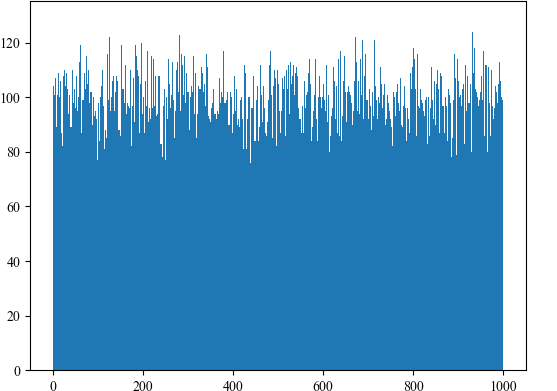
\includegraphics[width=.49\linewidth]{images/t_digest_data.png}
	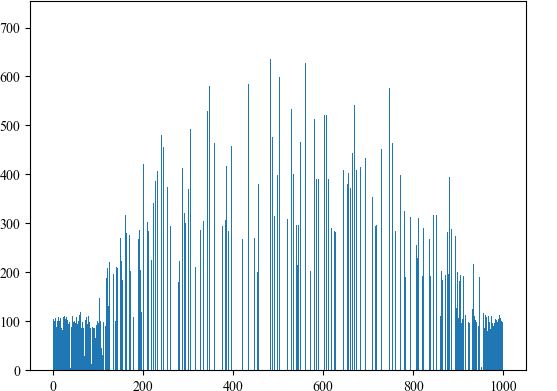
\includegraphics[width=.49\linewidth]{images/t_digest_sorted.png}
	\caption{Schwerpunktverteilung durch T-Digest}
	\label{fig:t-digest}
\end{figure}

In einem selbst durchgeführten Test, in dem eine Implementierung des T-Digest-Algorithmus mit einer einfachen, sortierten Liste verglichen wurde, hat sich die Präzision des T-Digest als sehr gut herausgestellt.
Es wurden 100\,000 verschiedene, zufällige Zahlen von 1 bis 1\,000 in beide Objekte eingetragen, wobei anschließend je der Median, sowie das 99,99\%-Quantil geprüft wurden.

Hierbei ergab sich, dass der Median zwar nur in 0,33\% der Fälle akkurat war, jedoch nie eine Abweichung von $\pm$\,0,5\% überschritt.
Für das 99,99\%-Quantil war der T-Digest in 99,79\% der Fälle akkurat, in den übrigen Fällen wies er eine Abweichung von maximal $\pm$\,0,01\% auf.

Außerdem hat sich die von Dunning und Ertl \cite{dunning2019} beschriebene, sehr hohe Geschwindigkeit bei diesem Test ebenso bewahrheitet.
Sowohl das Einfügen in die Liste, als auch in den T-Digest bewegt sich durchschnittlich in der gleichen Größenordnung von 10\textsuperscript{-5}\,Sekunden (10\,\textmu{}s).
Gleiches gilt für das identifizieren eines Quantils, was in beiden Fällen in der Größenordnung 10\textsuperscript{-4}\,Sekunden (100\,\textmu{}s) passiert.

Ein weiterer Vorteil des T-Digest-Algorithmus ist, dass die Daten mehrerer Digests einfach verbunden werden können, solange man die Gewichte der Schwerpunkte beachtet \cite{dunning2019}.
Dies ist zum Beispiel nützlich, wenn man einen Median aus mehreren, großen Datensätzen identifizieren möchte, da es hierfür nicht einfach reicht, den Median für jeden Datensatz einzeln zu identifizieren und aus der Liste der Ergebnisse einen neuen Median zu ziehen.


\subsection{Count-Min-Sketch}

Der Count-Min-Sketch ist ein Algorithmus von Cormode und Muthukrishnan \cite{cormode2005}, 
mit dem die Häufigkeit aller Elemente in einem Stream approximativ ermittelt werden kann. 
Die Häufigkeiten werden dabei in ein Array geschrieben, 
wodurch die benötigte Speichergröße für die Datenmenge stark komprimiert, 
aber dafür etwas ungenauer wird. 
Der Algorithmus weist für häufige Elemente eine hohe Genauigkeit auf 
und wird deshalb für die Ermittlung der Häufigkeit von Elementen genutzt, 
von denen erwartet wird, dass sie oft in dem Stream enthalten sind.

Um die Häufigkeit eines Elements zu ermitteln 
nutzt der Algorithmus ein Array mit mehreren Zeilen 
und ebenso viele verschiedene, paarweise unabhängige Hashfunktionen. \todo[inline]{was ist paarweise unabhängig?}
Jedes Element des Streams wird dann mit den Hashfunktionen gehasht 
und in die der Hashfunktion zugeteilte Zeile eingetragen. 
Wird ein Hashwert in einer Zeile mehrfach hinzugefügt, 
erhöht sich dann ein Counter für diesen Hashwert. 
Es kann passieren, dass für verschiedene Werte der selbe Hashwert erzeugt 
und so auch der gleiche Counter erhöht wird. 
Durch dieses Verhalten kann für einen einzelnen Hashwert 
schlussendlich nicht mehr unterschieden werden, 
wie hoch die Häufigkeit eines Elements unter diesem Hashwert ist. 
Es ergibt sich jedoch, dass der Hashwert des Elements, dessen Count am geringsten ist, 
durch die wenigsten Hashwerte anderer Elemente erhöht wurde. 
Somit ist der Hashwert des Elements mit dem geringsten Count der, 
der dem tatsächlichen Wert am nächsten kommt \cite{cormode2017}.

Der Aufbau des Algorithmus ähnelt dem des Bloom Filter Algorithmus \cite{cormode2017}. 
Das Array, das für den Bloom Filter Algorithmus verwendet wird, 
hat jedoch nur eine Zeile in die die gehashten Werte aller Hashfunktionen eingetragen werden \cite{cormode2017}.

Durch die Erhöhung der Menge verschiedener Hashfunktionen kann die Abweichung des Counts reduziert werden. 
Somit lässt sich durch Erhöhen oder Reduzieren der Menge an Hashfunktionen 
der Count-Min-Sketch dem Bedürfnis von Präzision oder Geschwindigkeit anpassen.

\subsection{StreamApprox}

StreamApprox ist ein Sampling Algorithmus der dafür entwickelt wurde, 
die Datenmenge eines Streams auf eine bestimmte Größe zu limitieren, 
indem er nur einige Daten des Streams weiterreicht. 
Dabei erfolgt die Selektierung, welche Daten weitergegeben werden, durch einen Zufallsalgorithmus. 
Auf diese Weise wird das Ergebnis der Auswertung des Streams weniger stark beeinträchtigt, 
als wenn die Daten, die die Verarbeitungskapazitäten überschreiten, 
überhaupt nicht betrachtet werden. 
Der Algorithmus ist dabei sowohl auf Batch-, als auch auf Pipeline-basierte Streams anwendbar.
Das besondere an StreamApprox ist die Fähigkeit, 
die Größe des Streams zu limitieren und dabei so wenig Daten wie möglich aus dem Stream zu entfernen. 
Der Algorithmus reduziert also nur dann den Datenstrom, wenn dessen Datenmenge ein eingestelltes Limit überschreitet. 
Diese Fähigkeit übersteigt die von Random Sampling Algorithmen, 
die für eine ähnliche Ausgabe die absolute Anzahl an Elementen des Streams kennen müssten. 
Ermöglicht wird das durch die Verwendung von sog. Reservoir Sampling, 
bei dem die Elemente des Streams in einen Pufferspeicher geschrieben werden, 
wobei neue Elemente an einer zufälligen Stelle des Puffers den vorherigen Wert überschreiben, sobald dieser voll ist \cite{quoc2017}. 

Dieses Vorgehen kann hilfreich sein, 
wenn die Datenmenge für die gewünschte Analyse stark variiert oder zu groß ist und reduziert werden soll, 
um eine bestimmte Verarbeitungsgeschwindigkeit beizubehalten, 
ohne das Ergebnis der Analyse zu stark zu beeinflussen.
Bei einer Entfernung der Daten mit einem Muster, zum Beispiel Überschreiben jedes zweiten Felds im Pufferspeicher, 
könnten so eventuelle Muster einkommender Daten stärker betroffen sein, als bei einem zufälligen Überschreiben.
Es kann ebenfalls hilfreich sein, 
wenn, aufgrund fehlender Ressourcen zur Verarbeitung, 
die Menge an gelieferten Daten reduziert werden soll.